\documentclass[spanish,a4paper,11pt,twoside]{report}
\usepackage[spanish]{babel}
\usepackage[utf8]{inputenc}
\usepackage{graphicx}

%%%%%%%%%%%%%%%%%%%%%%%%%%%%%%%%%%%%%%%%%%%%%%%%%%%%%%%%%%%%%%%%%%%%%%%%%%%%%%%

\newcommand{\SONY}{{\sc Sony}}
\newcommand{\MICROSOFT}{{\sc Microsoft}}
\newcommand{\GCC}{\textsf{\textsc{G}CC}}
\newcommand{\INTEL}{\textsf{\textsc{I}ntel}}

\newcommand{\RET}{\STATE \textbf{retornar} }
\newcommand{\TO}{\textbf{hasta} }
\newcommand{\AND}{\textbf{y} }
\newcommand{\OR}{\textbf{o} }

%Entorno para listar código fuente
\newenvironment{sourcecode}
{\begin{list}{}{\setlength{\leftmargin}{1em}}\item\scriptsize\bfseries}
{\end{list}}

\newenvironment{littlesourcecode}
{\begin{list}{}{\setlength{\leftmargin}{1em}}\item\tiny\bfseries}
{\end{list}}

\newenvironment{summary}
{\par\noindent\begin{center}\textbf{Abstract}\end{center}\begin{itshape}\par\noindent}
{\end{itshape}}

\newenvironment{keywords}
{\begin{list}{}{\setlength{\leftmargin}{1em}}\item[\hskip\labelsep \bfseries Keywords:]}
{\end{list}}

\newenvironment{palabrasClave}
{\begin{list}{}{\setlength{\leftmargin}{1em}}\item[\hskip\labelsep \bfseries Palabras clave:]}
{\end{list}}


%%%%%%%%%%%%%%%%%%%%%%%%%%%%%%%%%%%%%%%%%%%%%%%%%%%%%%%%%%%%%%%%%%%%%%%%%%%%%%%
% Formato de las páginas


%%\topmargin -4 mm
%\topmargin -21 mm
%\headheight 10 mm
%\headsep 10 mm

%\textheight 229 mm
%\textheight 246 mm

%\oddsidemargin -5.4 mm
%\evensidemargin -5.4 mm
\oddsidemargin 5 mm
\evensidemargin 5 mm

%\oddsidemargin -3 mm
%\evensidemargin -3 mm

%\textwidth 17 cm
\textwidth 15 cm
%\columnsep 10 mm

\input{amssym.def}

%%%%%%%%%%%%%%%%%%%%%%%%%%%%%%%%%%%%%%%%%%%%%%%%%%%%%%%%%%%%%%%%%%%%%%%%%%%%%%%

\begin{document}

%++++++++++++++++++++++++++++++++++++++++++++++++++++++++++++++++++++++++++
% Portada


\pagestyle{empty}
\thispagestyle{empty}


\newcommand{\HRule}{\rule{\linewidth}{1mm}}
\setlength{\parindent}{0mm}
\setlength{\parskip}{0mm}
\vspace*{\stretch{1}}



\HRule
\begin{center}
        {\Huge Interpolación de} \\[2.5mm] 
        {\Huge Taylor} \\[2.5mm]
        {\Large  Mérari Afonso \\ Ignacio Fragoso \\ Lidia García} \\[5mm]
        {\Large \textit{Grupo $1F$ }} \\[5mm]


        {\em Técnicas Experimentales. $1^{er}$ curso. $2^{do}$ semestre} \\[5mm]
        
        Facultad de Matemáticas \\[5mm]
        
        Universidad de La Laguna \\
\end{center}
\HRule
\vspace*{\stretch{2}}
\begin{center}
  La Laguna, \today 
\end{center}



%%%%%%%%%%%%%%%%%%%%%%%%%%%%%%%%%%%%%%%%%%%%%%%%%%%%%%%%%%%%%%%%%%%%%%%%
\newpage{\pagestyle{empty}\cleardoublepage}

\pagestyle{myheadings} 
\markboth{Nombre del alumno}{Interpolación de Taylor}

%%%%%%%%%%%%%%%%%%%%%%%%%%%%%%%%%%%%%%%%%%%%%%%%%%%%%%%%%%%%%%%%%%%%%%%%

\pagestyle{plain}
\setcounter{page}{1}

%%%%%%%%%%%%%%%%%%%%%%%%%%%%%%%%%%%%%%%%%%%%%%%%%%%%%%%%%%%%%%%%%%%%%%%%

\tableofcontents

%%%%%%%%%%%%%%%%%%%%%%%%%%%%%%%%%%%%%%%%%%%%%%%%%%%%%%%%%%%%%%%%%%%%%%%%
\newpage{\pagestyle{empty}\cleardoublepage} %Imagenes
\listoffigures









%%%%%%%%%%%%%%%%%%%%%%%%%%%%%%%%%%%%%%%%%%%%%%%%%%%%%%%%%%%%%%%%%%%%%%%%
%\newpage{\pagestyle{empty}\cleardoublepage} 
\listoftables % Tablas









%%%%%%%%%%%%%%%%%%%%%%%%%%%%%%%%%%%%%%%%%%%%%%%%%%%%%%%%%%%%%%%%%%%%%%%%%%%%%%%
%\newpage{\pagestyle{empty}\cleardoublepage}

%%%%%%%%%%%%%%%%%%%%%%%%%%%%%%%%%%%%%%%%%%%%%%%%%%%%%%%%%%%%%%%%%%%%%%%%%%%%%%%
\setlength{\parindent}{5mm}

%++++++++++++++++++++++++++++++++++++++++++++++++++++++++++++++++++++++++++
\chapter{Motivacion y objetivos}
\label{chapter:obj}
El objetivo de este trabajo principalmente ha sido desarrollar un experimento para evaluar la interpolación de Taylor de una función concreta. Para ello hemos desarrollado un programa en Python que calcula el polinomio de Taylor en un punto dado, la función real en el punto y el error que se comete al hallar el polinomio frente al valor real.



%++++++++++++++++++++++++++++++++++++++++++++++++++++++++++++++++++++++++++
\chapter{Fundamentos teóricos}
\label{chapter:teo}
%En este capítulo se han de presentar los antecedentes teóricos y prácticos que
%apoyan el tema objeto de la investigación.

	Para comprender de forma correcta el tema a exponer es necesario conocer primero la definición de interpolar. Según la Real Academia Española (RAE) disponemos de estas cuatro opciones: 
\begin{itemize}
  \item [$*$]
  Poner algo entre cosas.
  \item [$*$]
  Intercalar palabras o frases en el texto de un manuscrito antiguo, o en obras y escritos ajenos.
  \item [$*$]
  Interrumpir o hacer una breve intermisión en la continuación de algo, y volver luego a proseguirlo.
  \item [$*$]
  Calcular el valor aproximado de una magnitud en un intervalo cuando se conocen algunos de los valores que toma a uno y otro lado de dicho intervalo.\\
\end{itemize}


En nuestro caso, la opción que define mejor el tema a tratar es la última, ya que se trata de la definición matemática de interpolación.\\
La interpolación surge porque muchas veces en una función sólo conocemos un conjunto de valores, y si queremos calcular el valor de la función para una abscisa diferente de las conocidas, debemos utilizar otra función que la aproxime, por tanto el valor que obtengamos será una aproximación del valor real. Lo que nos lleva a estar cometiendo un error, ya que se trata de una aproximación.\\
Pese a que existen varias formas de realizar este cálculo, se utiliza la interpolación porque es el método más sencillo.\\
En este caso se utilizan polinomios como funciones de aproximación. Este tipo de interpolación se denomina interpolación polinómica.\\


\section{Tipos de interpolación polinómica}
\label{2:sec:1}
  La función de interpolación a encontrar dependerá, entre otras cosas, de la cantidad de datos reales de los que partimos, y de cómo estos puntos se distribuyen por el plano cartesiano. Esto nos dará una idea del tipo de función de interpolación que debemos buscar.

\subsection{Interpolación Lineal}
  Este tipo de interpolación es empleado cuando suponemos que las variaciones son proporcionales.\\
  Por ejemplo: 
Dados dos puntos ($x_1$, $y_1$) y  ($x_2$, $y_2$), entonces la interpolación lineal consiste en hallar una estimación del valor $y$, para un valor $x$  tal que $x_1<x <x_2$. Teniendo en cuenta estas suposiciones, podemos determinar:

\[
y = y_1 + \frac{(y_2 - y_1)(x - x_1)}{x_2 - x_1}
\]\\ 
\begin{figure}
\begin{center}
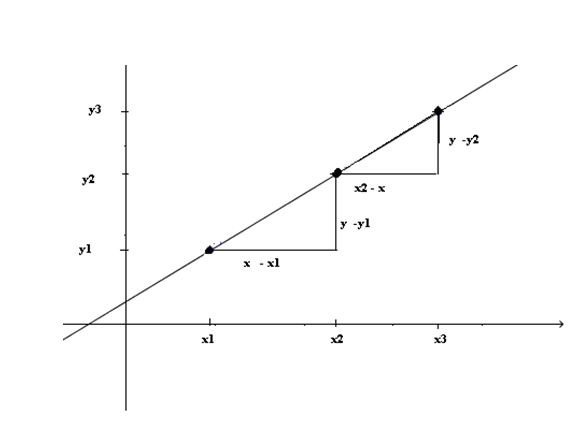
\includegraphics[scale=0.5]{grafica3.png}
\caption{Ejemplo 1.}
\label{Ejemplo 1}
\end{center}
\end{figure}


\subsection{Interpolación Cuadrática}
Si en vez de utilizar rectas, es decir polinomios de primer grado, utilizamos polinomios de segundo grado para interpolar, estaremos realizando interpolación cuadrática. Para la interpolación lineal utilizábamos dos puntos, ya que dos puntos determinan una recta, ahora necesitaremos tres puntos para determinar la correspondiente parábola.\\
El forma de resolver el sistema para encontrar los valores que determinan a la función cuadrática $(a, b, c)$ es:

\[
y = a + b(x - x_0) + c(x - x_0)(x - x_1)
\]\\

Lagrange ~\cite{Lagrange} expuso una manera simplificada de calcular los polinomios interpoladores de grado $n$ para el caso de un polinomio de 2º grado que pasa por los puntos $(x_0, y_0), (x_1, y_1), (x_2, y_2)$:\\

\[
y = y_0\frac{(x - x_1)(x - x_2)}{(x_0 - x_1)(x - x_2)} + y_1\frac{(x- x_0)(x - x_2)}{(x_1 - x_0)(x_0 - x_2)} + y_2\frac{(x - _0)(x - x_1)}{(x_2 - x_0)(x_2 - x_1)}
\]\\ 

A parte de la interpolación de Lagrange, existen otros métodos muy conocidos como son el método de las diferencias divididas de Newton y la interpolación de Hermite.\\
También existen métodos de Interpolación segmentaria que nos permiten aproximar funciones de un modo eficaz. Entre ellos cabe destacar la interpolación por splines y la interpolación de Taylor. Este último será el que estudiaremos nosotros.
\begin{verbatim}

\end{verbatim}

\begin{figure}[h]
\begin{center}
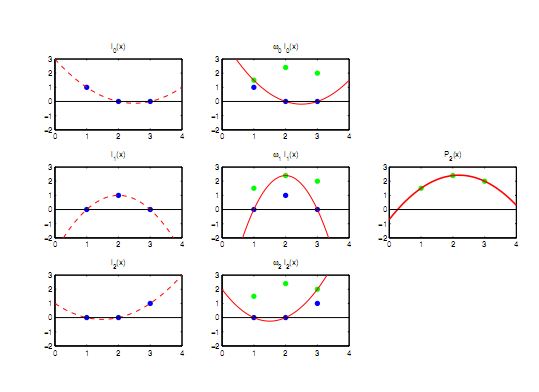
\includegraphics[scale=0.5]{graficalagrange.png}
\caption{Ejemplo 2.}
\label{Ejemplo 2}
\end{center}
\end{figure}
\section{Interpolación por Splines}
	La Interpolación por Splines es un refinamiento de la interpolación polinómica que usa "pedazos" de varios polinomios en distintos intervalos de la función a interpolar para evitar problemas de oscilación como el llamado Fenómeno de Runge.\\

La idea es que agrupamos las abscisas $x_0,x_1,...,x_m$ \ en distintos intervalos según el grado del spline que convenga emplear en cada uno. Así, un spline será un polinomio interpolador de grado n de f para cada intervalo. A la postre, los distintos splines quedarán "unidos" recubriendo todas las abscisas e interpolando a la función.\\

El principal problema que presenta la interpolación por splines reside en los puntos que son comunes a dos intervalos (extremos). Por esos puntos deben pasar los splines de ambos intervalos, pero para que la interpolación sea ajustada, conviene que el punto de unión entre dos splines sea lo más "suave" posible (ej. evitar puntos angulosos), por lo que se pedirá también que en esos puntos ambos splines tengan derivada común. Esto no será siempre posible y, a menudo, se empleará otro tipo de interpolación, quizás una interpolación no-polinómica.\\




\section{Interpolación  de Taylor}
\label{2:sec:2}
  La Interpolación de Taylor ~\cite{Taylor} usa el Desarrollo de Taylor de una función en un punto para construir un polinomio de grado $n$ que se aproxima a la función dada. Tiene dos ventajas esenciales sobre otras formas de interpolación:
  \begin{enumerate}
  \item
  Requiere sólo de un punto $X_0$ conocido de la función para su cálculo.
  \item
  El cálculo del Polinomio de Taylor es sumamente sencillo comparado con otras formas de interpolación polinómica:
  \end{enumerate}

\begin{center}
$P(x)=\sum\limits_{i=1}^n\frac{f^{(i)} (x_0)}{i!}\quad(x - x_0)^i $
\end{center} 
Sin embargo, el error que se comete al resolver este polinomio puede alcanzar cotas demasiado elevadas.\\
Para hallar el error restamos el valor real de la función menos el valor de la interpolación de Taylor en valor absoluto.\\
Sea p el valor real, y $p*$ el valor obtenido de realizar la interpolación, tenemos que el error es: $|p-p*|$\\
\begin{figure}[h]
\begin{center}  
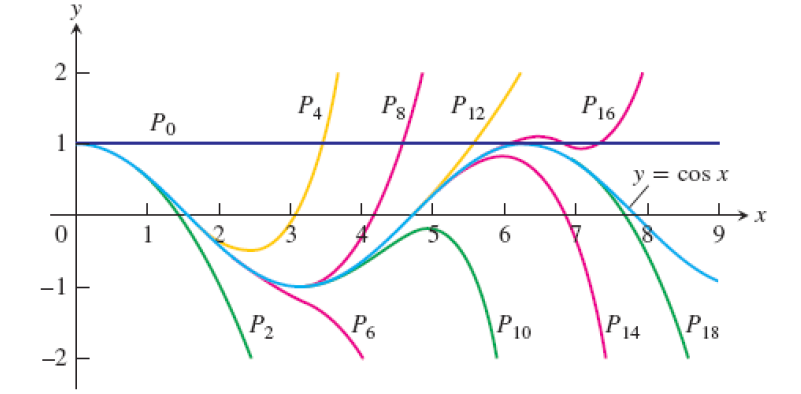
\includegraphics[scale=0.5]{grafica4.png} 
\caption{Ejemplo 3.}
\label{Ejemplo 3}
\end{center}  
\end{figure}
%++++++++++++++++++++++++++++++++++++++++++++++++++++++++++++++++++++++++++
\chapter{Procedimiento experimental}
\label{chapter:exp}
	Para realizar los pertinentes experimentos hemos creado un programa en lenguaje Python que nos proporciona de forma rápida y eficaz el resultado real, el resultado de realizar la interpolación de Taylor y el error que este método nos proporciona.\\ 
Estos resultados varían dependiendo del valor de x, el valor del centro ($x_0$  o c) y el valor de n que tomemos. Ya que el error que se comete es lo que nos define si la interpolación es válida y ya que éste ha sido el incentivo para realizar el trabajo, hemos realizado una serie de tablas acompañadas de gráficas que nos permiten ver de una forma clara qué sucede al variar el centro, la x o la n.\\
	Fijando el valor de x y la derivada n-ésima (x=1, n=5)\\
    \begin{table}[h]
	\begin{center}
	\begin{tabular}{||c|c|c|c||}
	\hline
    \hline
	Centro & Interpolación Taylor & Valor Real & Error \\
	\hline
	1.0 & -1 & -1 & 0\\
	\hline
	1.25 & -1.00025363221339 & -1 & 0.000253632213394583 \\
	\hline
	1.5 & -1.00452485553482 & -1 & 0.00452485553481630\\	
	\hline
	1.75 & -0.900045035338955 & -1 & 0.0999549646610447\\
	\hline
	2 & 0.123909925872083 & -1 & 1.12390992587208\\
	\hline
    \hline
    \end{tabular}
    \caption{Tabla 1.}
    \label{Tabla 1}
	\end{center}
	\end{table}\\
En este cuadro podemos observar como al ir incrementando el valor del centro (dentro del intervalo, por supuesto) el error incrementa notablemente.\\
 Para verlo gráficamente: \\


En el siguiente caso hemos fijado el centro en 1.5 y la n-ésima =  1\\
\begin{table}[h]
    \begin{center}
	\begin{tabular}{||c|c|c|c||}
	\hline
    \hline
	x & Int. Taylor & Valor Real & Error \\
	\hline
	-1.5 & -352.175700107991 & -1.8369701e-16 & 352.1757 \\
	\hline
	0.0 & -3.40445153931272 & 1 & 4.4044515393127 \\
	\hline
	1.0 & -1.00025363221339 & -1 & 0.00025363221339458\\	
	\hline
    1.5 & -0.000202346334410 & -1.8369701e-16 & 0.00020234633441002\\
    \hline
    3 & -3.03724338394450 & -1 & 2.0372433839445\\
    \hline
    \hline
	\end{tabular}
    \end{center}
    \caption{Tabla 2.}
    \label{Tabla 2}
\end{table}\\
\begin{verbatim}




\end{verbatim}




En esta ocasión podemos decir que no existe una pauta definida, es decir, no podemos decir que al aumentar x disminuya o aumente el error, o viceversa, pero sí podemos observar algo curioso: tomando valores de x que coinciden con el intervalo el error cometido es bastante menor que al tomar valores fuera de éste, pese a que estos valores no sean desmesurados, por ejemplo con x=-1.5 el error que se produce es de 352,1757.\\
Para apreciarlo mejor:\\


Por último, hemos realizado varios experimentos dejando fijo el centro y la x (c=1.5 y x=1):\\
	\begin{table}[h]
	\begin{center}
	\begin{tabular}{||c|c|c|c||}
	\hline
    \hline
	n-ésima & Interpolación Taylor & Valor Real & Error \\
    \hline
	3 & -0.924832229288648 & -1 & 0.075167770711351\\
	\hline
    8 & -0.99984
    3101399498 & -1 & 0.000156898600502386\\
    \hline
    10 & -1.00000354258429 & -1 & 3.54258428503229e-6 \\
    \hline
    17 & -1.00000000000004 & -1 & 4.26325641456060e-14\\
	\hline
	20 & -0.999999999999999 & -1 & 1.1102302462516e-15\\	
	\hline
    \hline
	\end{tabular}
	\end{center}
    \caption{Tabla 3.}
    \label{Tabla 3}
    \end{table}
\begin{verbatim}


\end{verbatim}

	Esta vez se puede apreciar claramente como al aumentar la n-ésima el error se reduce hasta llegar a un valor de 1.1102302462516e-15, valor que curiosamente se mantiene constante a partir de n=20.\\
Para reflejarlo mejor hemos decidido hacer dos gráficas, la primera nos muestra la variación entre los valores que toma la función real y los valores que toma la interpolación de Taylor para n=2. En la segunda gráfica hemos aumentado esta n y podemos observar como prácticamente no existe variación entre las dos funciones

\begin{figure}
\begin{center}
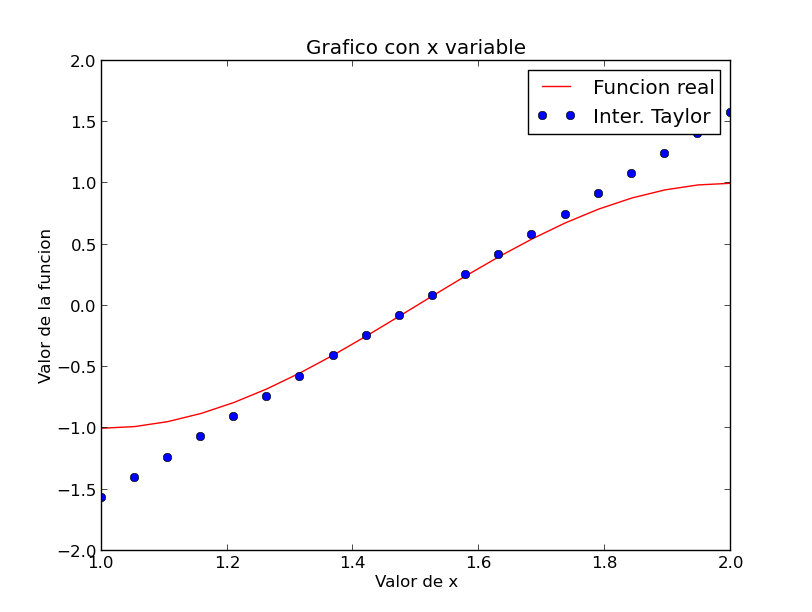
\includegraphics[scale=0.5]{grafica1.png}
\caption{Gráfica 1.}
\label{Grafica1}
\end{center}
\end{figure}

\begin{figure}
\begin{center}
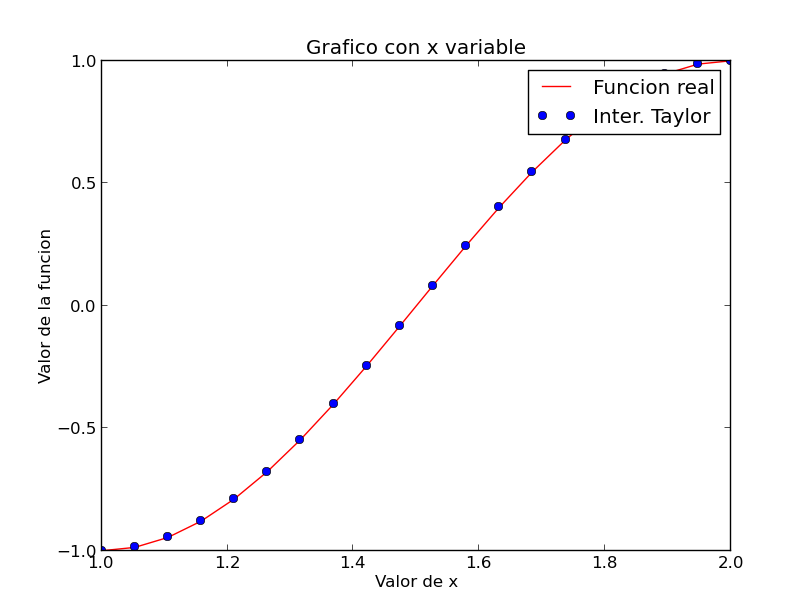
\includegraphics[scale=0.5]{grafica2.png}\label{Grafica2}
\caption{Gráfica 2.}
\end{center}
\end{figure}
%\input{tex/cap3.tex}

%%%%%%%%%%%%%%%%%%%%%%%%%%%%%%%%%%%%%%%%%%%%%%%%%%%%%%%%%%%%%%%%%%%%%%%%
\chapter{Conclusiones}
\label{chapter:conclusiones}

	Tiene dos ventajas esenciales sobre otras formas de interpolación: \\
Requiere sólo de un punto $x_0$ conocido de la función para su cálculo, 
si bien se pide que la función sea suficientemente diferenciable en un 
entorno de ese punto.\\
El cálculo del polinomio de Taylor es sumamente sencillo comparado con 
otras formas de interpolación polinómica.\\
Sin embargo, en ocasiones no será deseable su uso, dado que el error de 
interpolación puede alcanzar cotas demasiado elevadas. En nuestro caso 
particular, el método funcióna bien ya que se trata de una función 
continua y cuyas derivadas son fáciles de calcular.\\
tomamos un polinomio de orden alto el error que cometemos al realizar la 
interpolación es prácticamente nulo, mientras que al tomar polinomios 
con un orden pequeño solo escasos valores tendran semejanza con el valor 
real de la función.\\
%\input{tex/cap4.tex}

%++++++++++++++++++++++++++++++++++++++++++++++++++++++++++++++++++++++++++


%\newpage{\pagestyle{empty}\cleardoublepage}
%\thispagestyle{empty}
\begin{appendix}
\chapter{Ápendice}
\label{appendix}
\section{Programa Python}
\label{Apendice1:XXX}

\begin{center}
\begin{footnotesize}
\begin{verbatim}
#!/usr/bin/python 
import random, sys
from sympy import *

valor_c = Symbol('c')
pi = 3.141592653589793238462643383279502884197169399375105820974944592307816406286
funcion = cos(pi*valor_c)

def fac(n):
  if n == 0:
    return 1 
  else:
    return n * fac(n-1)

def Taylor(x,c,n):
  polinomio = 0
  for i in range(n + 1):
    derivada = eval(str(diff(funcion,valor_c,i)))
    polinomio += ((derivada/(fac(i)))*((x - c)**i))
  return polinomio

def real(x):
  resultado = eval(str(cos (pi*x)))
  return resultado

if __name__=='__main__': 
  x=float(sys.argv[1])
  c=float(sys.argv[2])
  n=int(sys.argv[3])
  print "El resultado de evaluar la derivada {0}-esima en el punto {1}, cuyo centro es {2} es {3}".format(n, x, c, Taylor(x,c,n))
  print "El valor real de la funcion en el punto {0} es: {1}".format(x, real(x))
  print "El error es ", abs(real(x)-Taylor(x,c,n))
\end{verbatim}
\end{footnotesize}
\end{center}

\section{Programa python de las gráficas}
\label{Apendice1:YYY}
\begin{center}
\begin{footnotesize}
\begin{verbatim}
- Gráfica para representar 20 puntos entre [1,2] fijando los valores de
la n-ésima (n=2) y el valor del centro (c=1.5)


from matplotlib.pylab import *
from math import *
from sympy import *

x=linspace(1,2,20)
pi = 3.141592653589793238462643383279502884197169399375105820974944592307816406286
sym_c = Symbol('c')
c = 1.5
n = 2

def f1(x):
  funcion = []
  for i in x:
    funcion.append(cos(pi*i))
  return funcion

def fac(n):
  if n == 0:
    return 1 
  else:
    return n * fac(n-1)

def f2(x):
  funcion = cos(pi*sym_c)
  polinomio = []
  for h in x:
    suma = 0
    for i in range(n + 1):
      derivada = eval(str(diff(funcion,sym_c,i)))
      suma += ((derivada/(fac(i)))*((h - c)**i))
    polinomio.append(suma)
  return polinomio

y1 = f1(x)
y2 = f2(x)


p1, = plot(x,y1,'r-')
p2, = plot(x,y2,'bo')
xlabel('Valor de x')
ylabel('Valor de la funcion')
legend([p1, p2], ['Funcion real', 'Inter. Taylor'])
title('Grafico con x variable')
xlim(1.0, 2.0)
show()



- Gráfica para representar 20 puntos entre [1,2] fijando los valores de
la n-ésima (n=20) y el valor del centro (c=1.5)


from matplotlib.pylab import *
from math import *
from sympy import *


x=linspace(1,2,20)
pi = 3.141592653589793238462643383279502884197169399375105820974944592307816406286
sym_c = Symbol('c')
c = 1.5
n = 20


def f1(x):
  funcion = []
  for i in x:
    funcion.append(cos(pi*i))
  return funcion

def fac(n):
  if n == 0:
    return 1 
  else:
    return n * fac(n-1)

def f2(x):
  funcion = cos(pi*sym_c)
  polinomio = []
  for h in x:
    suma = 0
    for i in range(n + 1):
      derivada = eval(str(diff(funcion,sym_c,i)))
      suma += ((derivada/(fac(i)))*((h - c)**i))
    polinomio.append(suma)
  return polinomio

y1 = f1(x)
y2 = f2(x)


p1, = plot(x,y1,'r-')
p2, = plot(x,y2,'bo')
xlabel('Valor de x')
ylabel('Valor de la funcion')
legend([p1, p2], ['Funcion real', 'Inter. Taylor'])
title('Grafico con x variable')
xlim(1.0, 2.0)
show()

\end{verbatim}
\end{footnotesize}
\end{center}

%++++++++++++++++++++++++++++++++++++++++++++++++++++++++++++++++++

\begin{thebibliography}{00}
  \bibitem{Taylor}
     Brook Taylor, (1685 - 1731), Nacionalidad Inglesa, Campo: Matemáticas, Conocido por: Teorema de Taylor, Serie de Taylor

  \bibitem{Lagrange}
  	Joseph-Louis Lagrange,
    (1736 - 1813),
    Nacionalidad Italiano Francés, Campo:Matemáticas,Física, matemática. Instituciones:	École polytechnique. Conocido por: Mecánica analítica, Mecánica celeste, Análisis matemático, Teoría de números.
 \end{thebibliography}
\end{appendix}
%%%%%%%%%%%%%%%%%%%%%%%%%%%%%%%%%%%%%%%%%%%%%%%%%%%%%%%%%%%%%%%%%%%%%%%%
\addcontentsline{toc}{chapter}{Bibliografía}
\bibliographystyle{plain}

{\small $http://www.slideshare.net/taker85/interpolacion-de-taylor-y-hermite$}\\
{\small $http://www.acm.org/publications/latex\_style/$}\\
{\small $http://www.ctan.org/$}
    



%\bibliography{bib/references}
\nocite{*}



%%%%%%%%%%%%%%%%%%%%%%%%%%%%%%%%%%%%%%%%%%%%%%%%%%%%%%%%%%%%%%%%%%%%%%%%%%%%%%%
\end{document}
